\documentclass[a4paper,11pt]{report}
\usepackage{amsmath}
\usepackage{graphicx}
\usepackage{wrapfig}
\usepackage{caption}
\usepackage{enumitem}
\usepackage{pdfpages}
\usepackage{multicol}
\usepackage[a4paper, left=3cm, right=3cm, top=3cm, bottom=3cm]{geometry}
\usepackage[ngerman]{babel}
\usepackage{hyperref}
\usepackage[x11names]{xcolor}
\usepackage{fancyhdr}
\pagestyle{fancy}
\usepackage{tikz}
\usetikzlibrary{calc}
\usepackage{titling}
\usepackage{fontspec}
\usepackage{titlesec}
\usepackage{moresize}
\usetikzlibrary{circuits.ee.IEC}

% font setup
\newfontfamily{\newUpperTitleFont}{Bebas Neue}
\newfontfamily{\newLowerTitleFont}{Tex Gyre Heros Bold}

% font init
\titleformat{\part}[display]{\centering\HUGE\scshape\newUpperTitleFont\color{SlateBlue4}}{\partname~\thepart}{10pt}{}
\titleformat{\chapter}{\Huge\bfseries\newUpperTitleFont\color{SlateBlue4}}{\thechapter}{1em}{}
\titleformat*{\section}{\Large\bfseries\newLowerTitleFont\color{SlateBlue3}}
\titleformat*{\subsection}{\large\bfseries\newLowerTitleFont\color{SlateBlue2}}
\titleformat*{\subsubsection}{\bfseries\newLowerTitleFont\color{SlateBlue1}}

% hyperlink setup
\hypersetup{
    colorlinks,
    citecolor=black,
    filecolor=black,
    linkcolor=SlateBlue3,
    urlcolor=black
}

% clear Footer
\fancyfoot{}

% Header
\fancyhead[L]{Andrin Tim Lerjen, \\ Nadja Rahm, Niklas Fister}
\fancyhead[C]{Kantonnschule - Physik}
\fancyhead[R]{\thepage}
\renewcommand{\headrulewidth}{1pt}
\setlength{\headheight}{30pt}

\fancypagestyle{plain}{
    \fancyhead[L]{Andrin Tim Lerjen, \\ Nadja Rahm, Niklas Fister}
    \fancyhead[C]{Kantonnschule - Physik}
    \fancyhead[R]{\thepage}
    \renewcommand{\headrulewidth}{1pt}
}

% Title
\title{\Huge\textbf{Bericht Physik - Lautsprecher}}
\author{Andrin Tim Lerjen, Nadja Rahm, Niklas Fister}
\date{\today}

% makeing title
\begin{document}
\pagenumbering{Roman}

% pretitle
%
\includepdf[scale=1.05]{resources/pdf/Title.pdf}

% own title
\begin{titlepage}
    \centering
    \begin{tikzpicture}[remember picture, overlay]
        \draw[line width=5pt, line cap=round, color=SlateBlue1, rounded corners=5pt]($(current page.west)+(1cm, 0)$) -- ($(current page.north west)+(1cm, -1cm)$) -- ($(current page.north)+(0, -1cm)$);
        \draw[line width=5pt, line cap=round, color=SlateBlue1, rounded corners=5pt]($(current page.east)+(-1cm, 0)$) -- ($(current page.south east)+(-1cm, 1cm)$) -- ($(current page.south)+(0, 1cm)$);
    \end{tikzpicture}

    % background
    \tikz[remember picture,overlay] \node[opacity=0.3,inner sep=0pt] at (current page.center){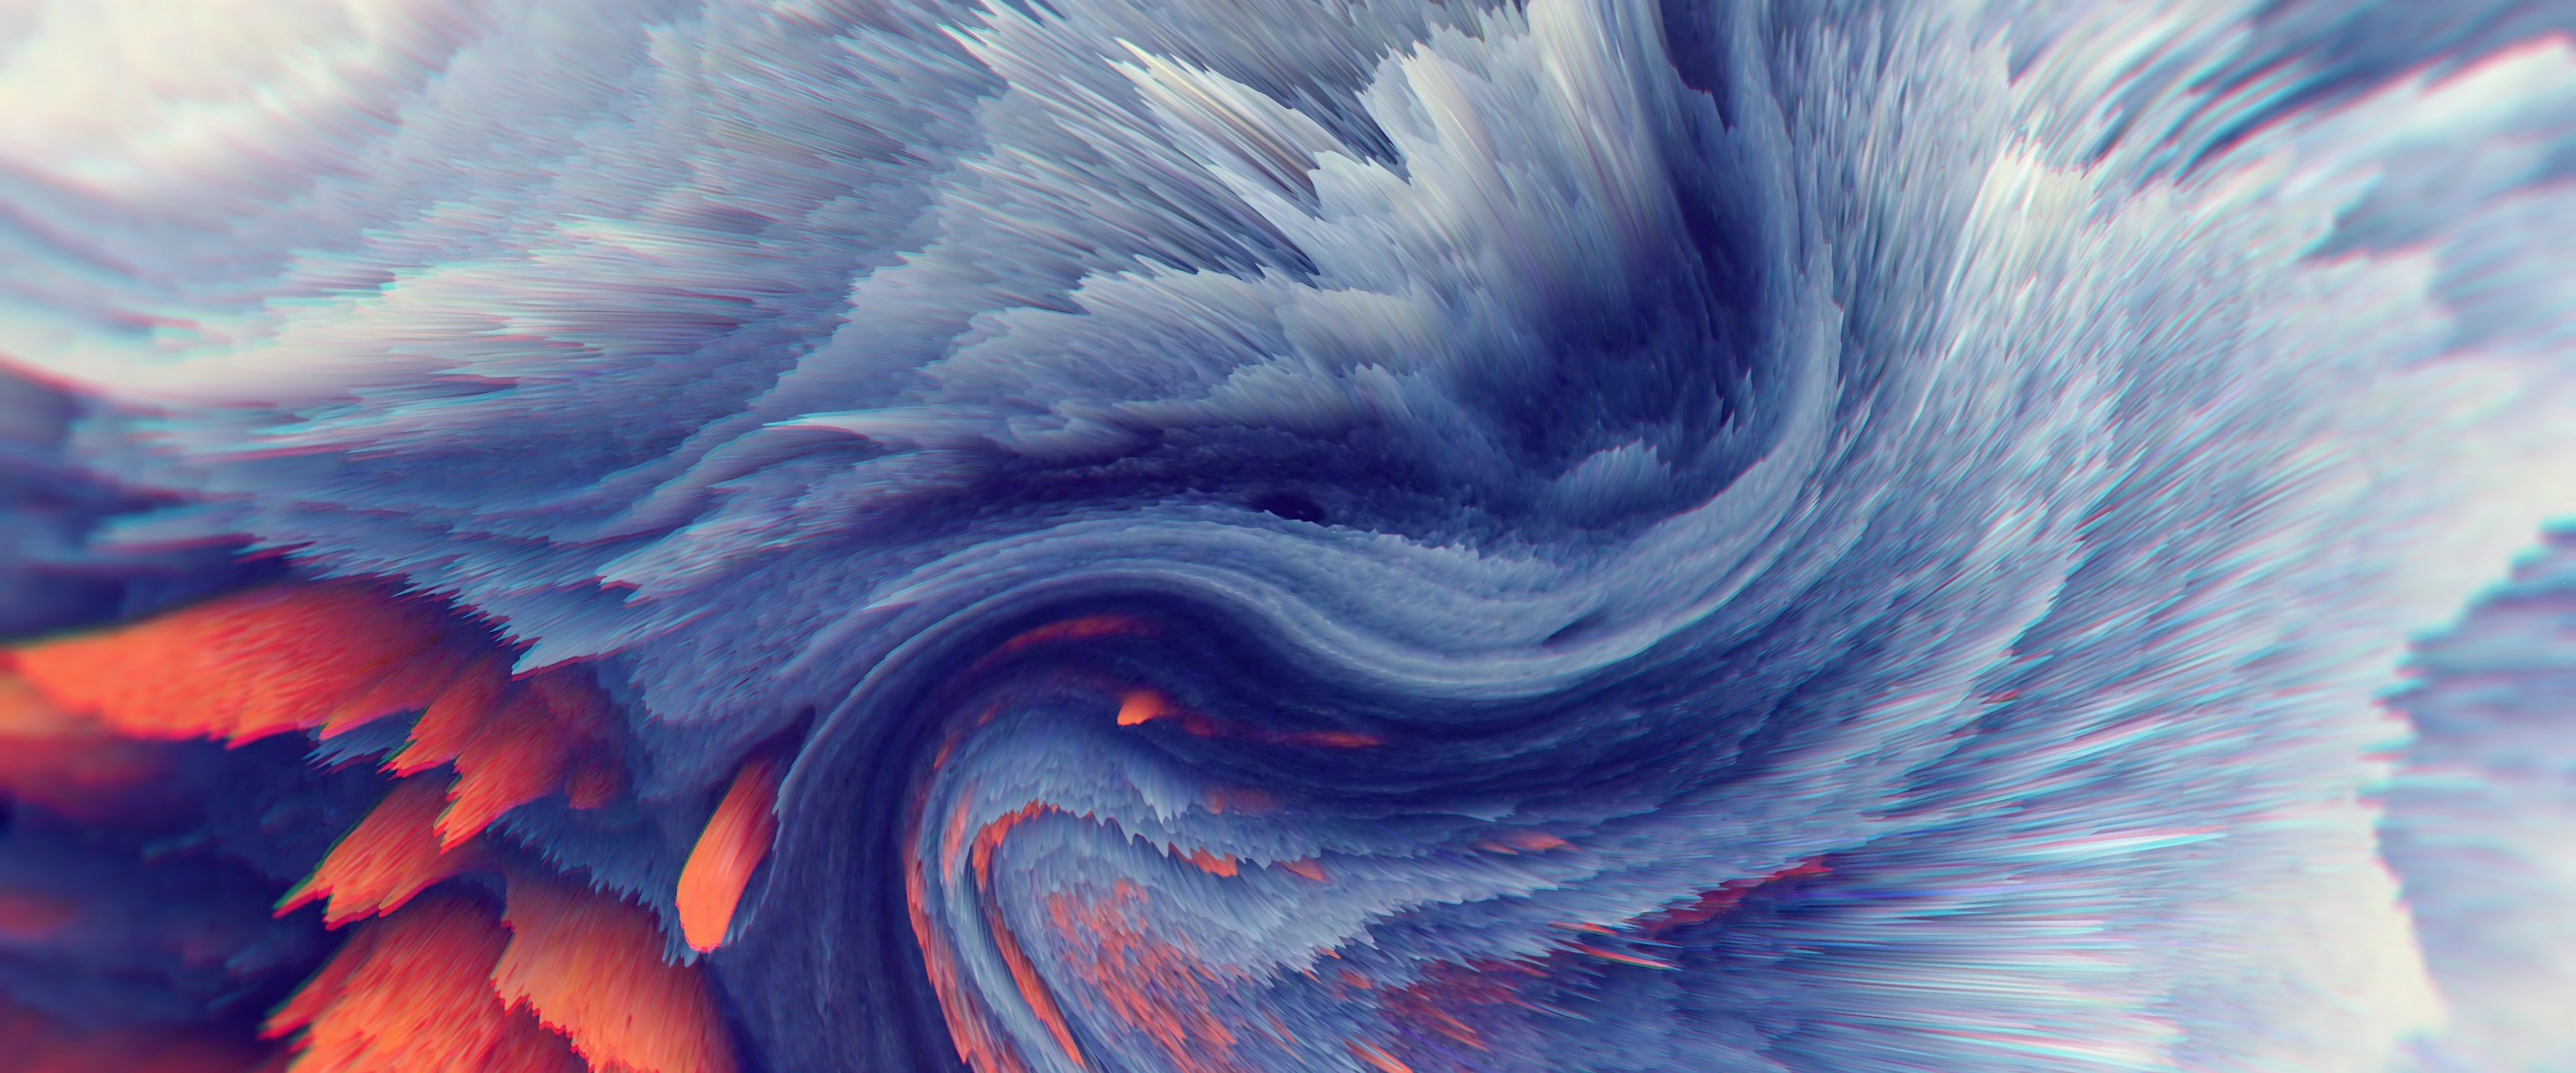
\includegraphics[width=\paperwidth - 4cm, height=\paperheight - 4cm]{resources/images/soundwave.jpg}};
    % Start Text
    \vspace{4cm}

    % the title
    {\newUpperTitleFont\thetitle\par}
    \vspace{1cm}

    % the autors
    {\theauthor\par}
    \vspace{.5cm}

    % date
    {\thedate\par}
    \vspace{5cm}

    % showcase
    %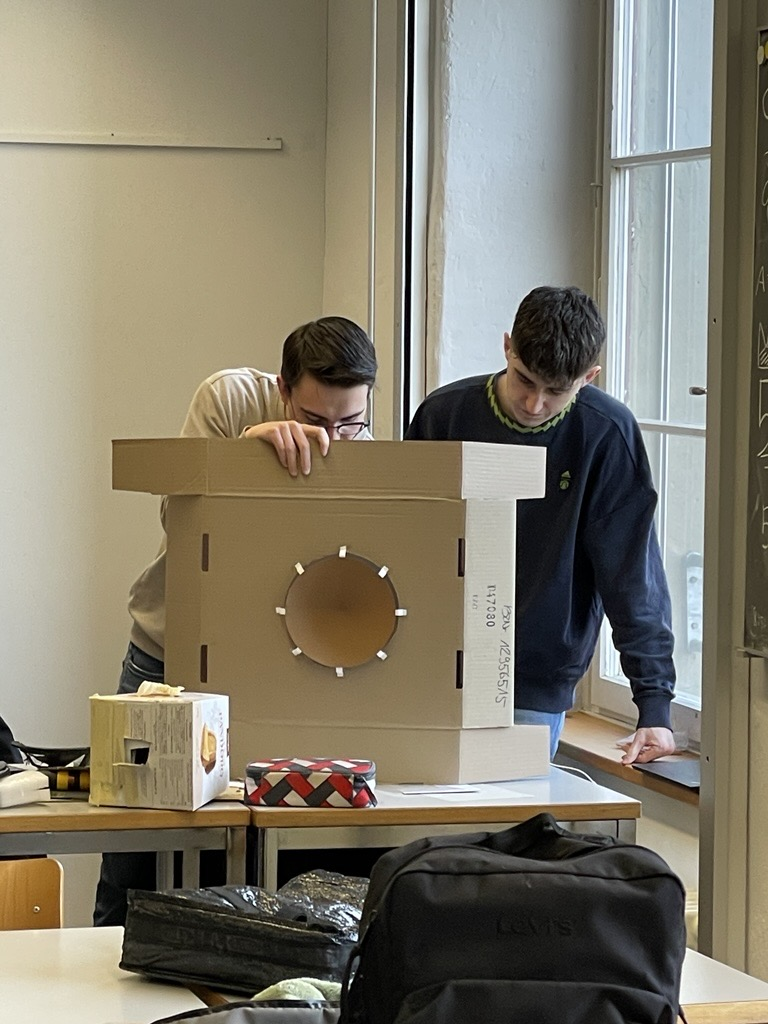
\includegraphics[width=.4\linewidth]{resources/images/Andrin_Cyrill_building.jpeg}
\end{titlepage}

% normal title
%\maketitle

% Abstract
\begin{abstract}
    In dem folgenden Bericht geht es um die Bau eines Lautsprechers aus alltäglichen Materialien.

    Es wurde ein leistungsstarker Lautsprecher gebaut, was vor allem an den starken Magneten liegt.

    Die Bauart aus leichten Materialien für den Schallerzeuger und dem stabilen Klangkörper sorgen für ein gutes Klangerlebnis.
    
\end{abstract}

% Table of contents
\tableofcontents
\thispagestyle{empty}

% report
\pagenumbering{arabic}
\setcounter{page}{1}

% Bericht
\part{Bericht}

% Introduction
\chapter{Einleitung}
\section{Fragestellung}
\begin{enumerate}
    \item Ist es möglich in der Schule einen gut funktionierenden Lautsprecher zu bauen?
    \item Ist es sinvoller einen Magneten innerhalb der Spule oder ausserhalb zu positionieren?
    \item Empfiehlt sich ein dickerer oder dünnerer Draht?
\end{enumerate}
\section{Hypothese}
\begin{enumerate}
    \item Wir gehen davon aus, dass wir einen Lautsprecher bauen können, der bei mittleren Lautstärken funktioniert, aber Schwächen bei sehr lauten Tönen und Bässen hat.
    \item Wir gehen davon aus, dass es sinvoller ist den Magneten ausserhalb der Spule zu positionieren.
    \item Wir gehen davon aus, dass ein dicker Draht sinvoller ist, da er weinger Widerstand hat und somit weniger Wärme erzeugt.
\end{enumerate}

\newpage
\section{Theorie}
\subsection{Wichtige Formeln}
\textbf{Relevante Variablen} \par
\begin{tabbing}
    gamma\quad\= a Greek latter\kill
    \(\mu_0\) :     \> magnetische Permeabilität des Vakuums \\
    \(\mu_r\) :     \>magnetische Permeabilität des Füllmaterials \\
    \(N\) :         \> Anzahl Windungen \\
    \(I\) :         \>Stromstärke \\
    \(L\) :         \>Länge der Spule \\
\end{tabbing}

\textbf{Berechnung der magnetischen Permeabilit im Vakuum}
\begin{equation}
    \mu_0 = 4 \cdot \pi \cdot 10^{-7} \frac{V \cdot s}{A \cdot m}
\end{equation}\par

\textbf{Berechnung der magnetischen Kraft mit Füllmaterial}
\begin{equation}
    B(r) \approx \frac{\mu_0 \cdot \mu_r \cdot N \cdot I}{L}
\end{equation}\par

\subsection{Geschichte des Lautsprechers}

\begin{wrapfigure}{r}{0.4\textwidth}
    \centering
    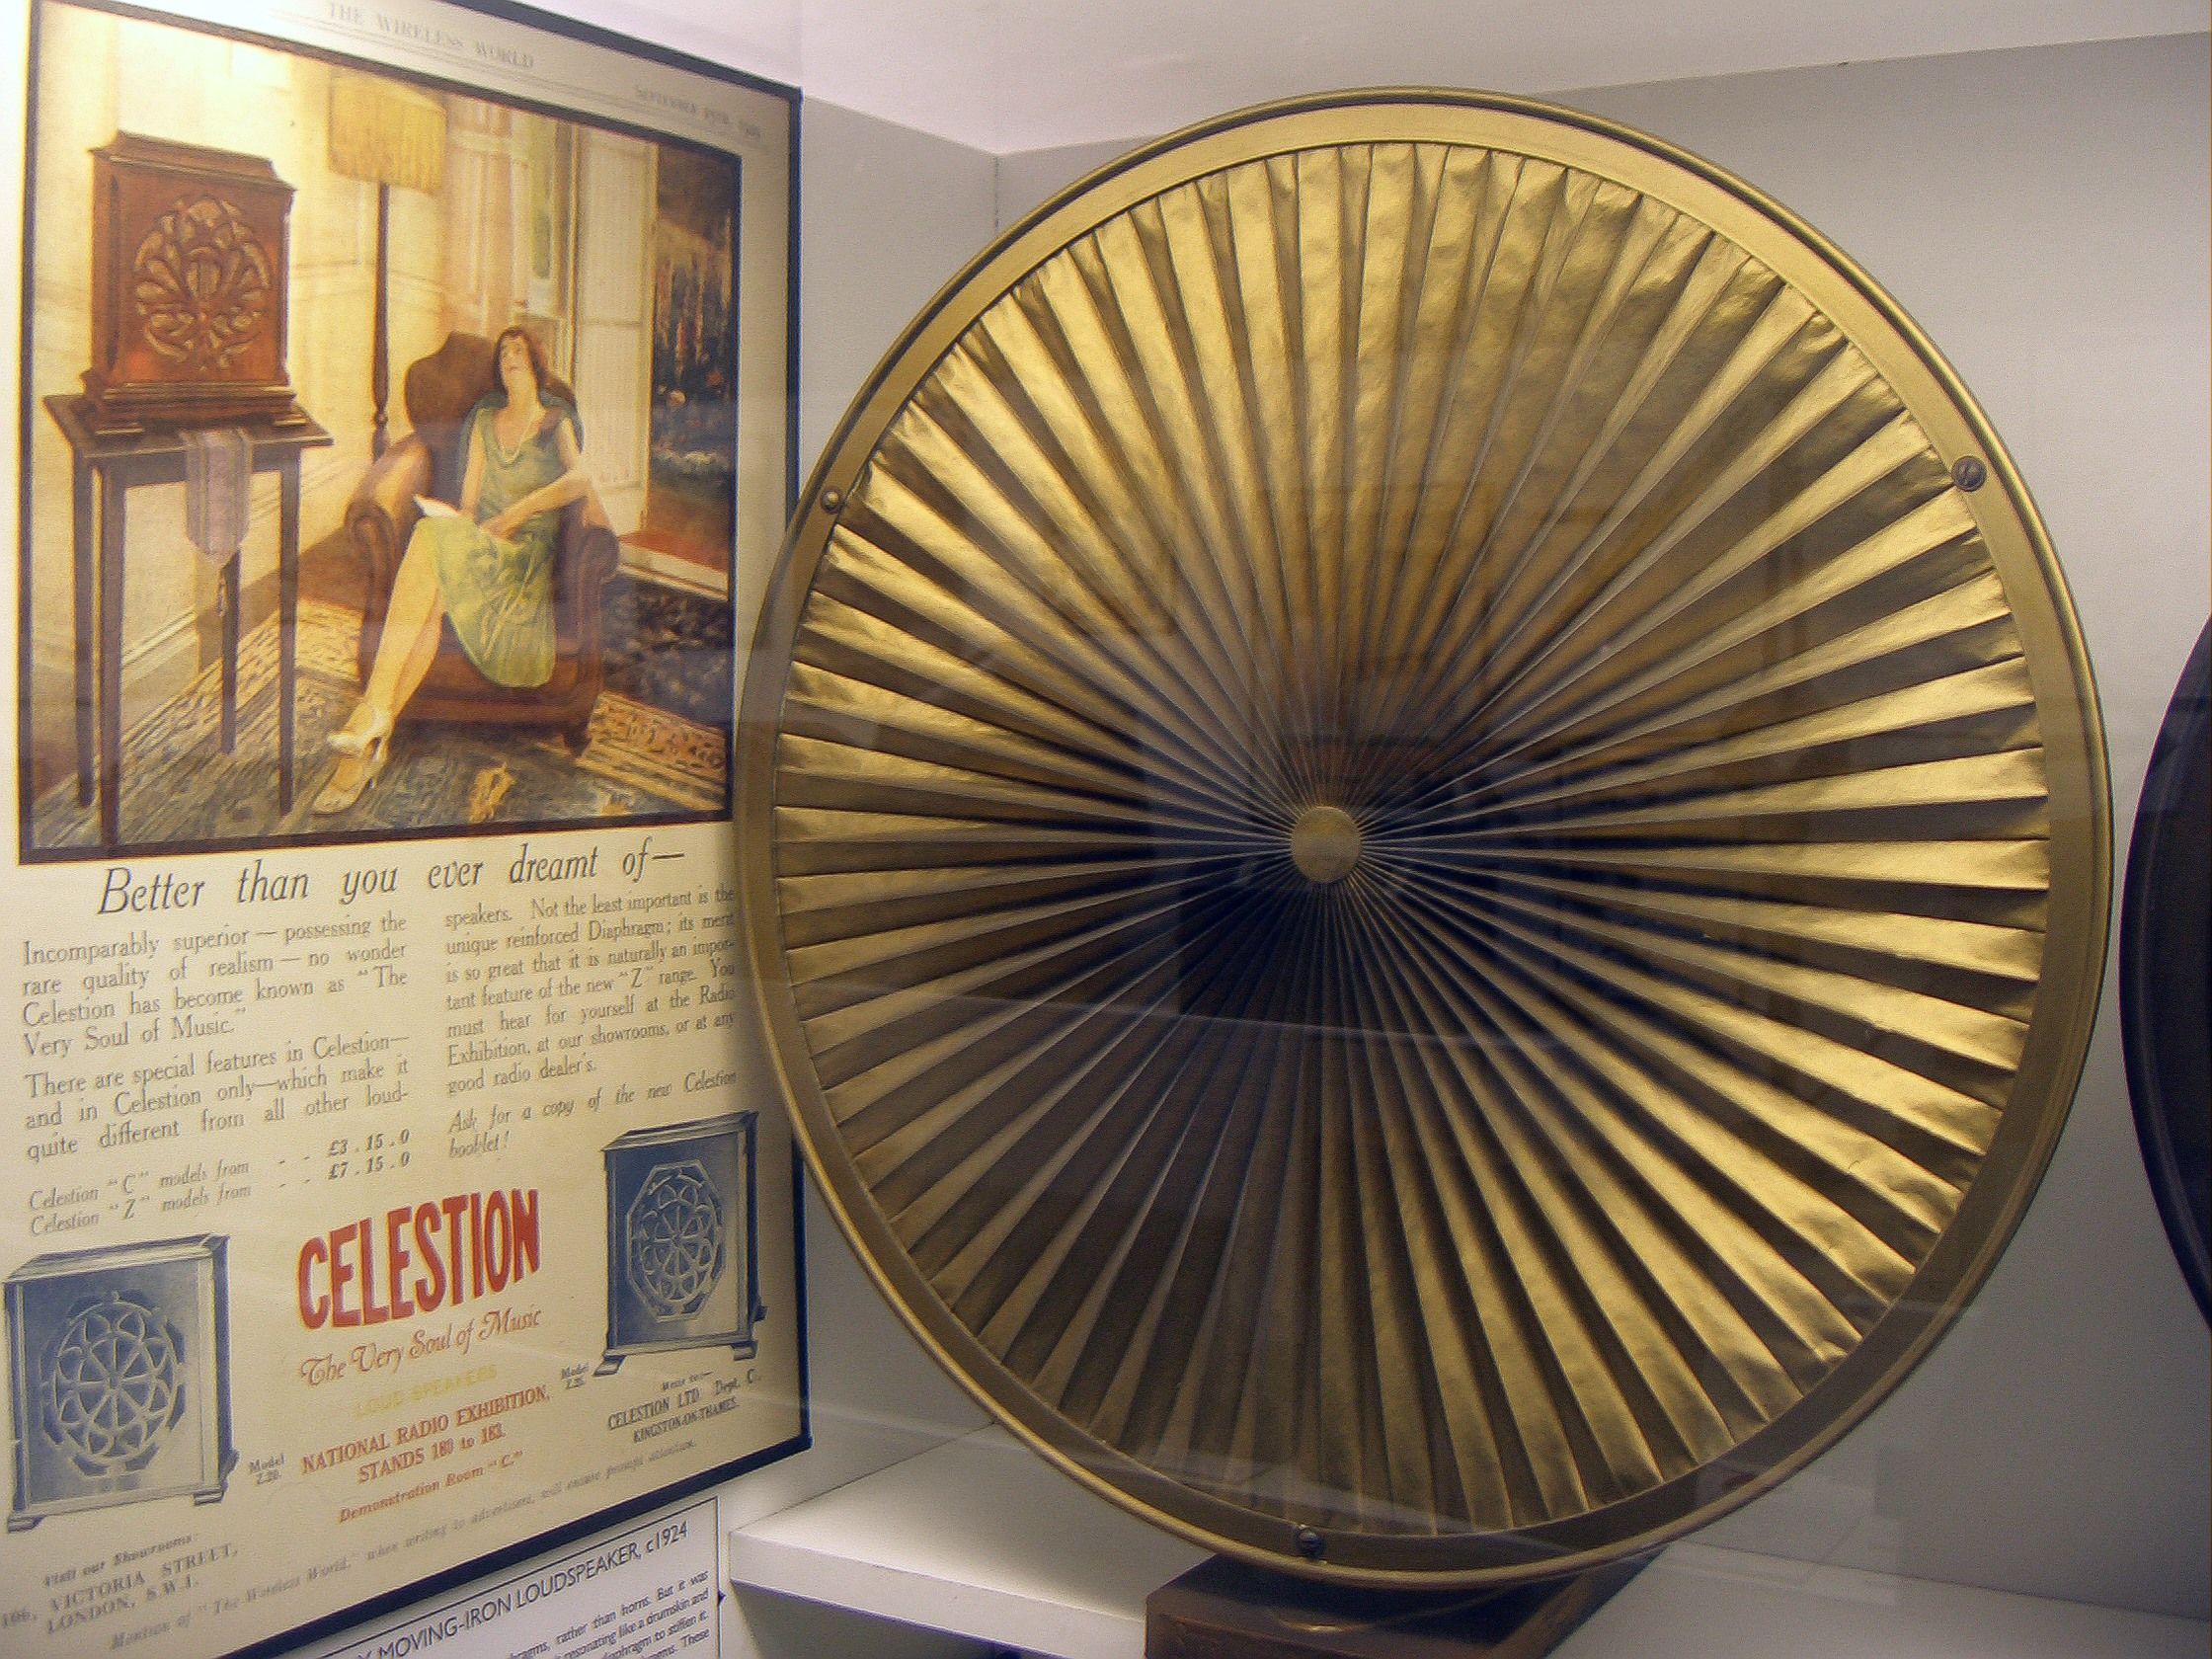
\includegraphics[width=.95\linewidth]{resources/images/Lautsprecher_Celestion.jpg}
    \caption{\raggedright{Lautsprecher von Celestion}}
    \label{fig:celection_speaker}
\end{wrapfigure}

Der Lautsprecher wurde im Jahre 1861 als mechanisches Nebenprodukt des Telefons entwickelt.

1878 wurde dann das Patent zu einem elektrischen Lautsprecher eingereicht, welches letztlich erst 1925 präsentiert wurde.
Das Grundprinzip blieb bis heute unverändert und ist in den Meisten Lautsprechern Vorzufinden. \cite{history_wikipedia}

Aufgrund der damaligen Bauart waren die Lautsprecher meinst sehr gross. Dies war Aufgrund der weichen Einspannung. \cite{history_connect}

Einen Entwickler für den Lautsprecher kann man jedoch nicht genau nennen, da es eine fliessende Entwicklung war, welche zum dem Produkt führten.

Vielen forschten gleichzeitig in diesem Thema und Patente unterschieden sich nur wage. Teils waren die Patente in den USA und Deutschland sogar nahezu identisch.\cite{history_tu_berlin}

% How to build it properly
\newpage
\subsection{Ideale Bauweise}
\subsubsection*{Bassreflexgeäuse}
\vspace{.5cm}
\noindent \begin{minipage}{0.6\textwidth}
    Um eine möglichst guten Bass zu generieren ist die Bauart eines Bassreflex-Gehäuses optimal. Durch die offene Bauweise mit einem sogenannten "Bassrefelexkanal" versehen.
    Das Innere des Körpers wird als Resonator gebraucht, um den Bass zu verstärken.
\end{minipage}
\hspace{0.1\textwidth}
\begin{minipage}{0.2\textwidth}
    \includegraphics[width=.9\textwidth]{resources/images/Bassreflex-Gehäuse.png}
    \captionof{figure}{\raggedright Bassreflex-Gehäuse}
    \label{fig:bass-reflex}
\end{minipage}
\vspace{.5cm}

Dabei wird als allgemeine Formel für die Berechnung der Resonator-Kanälen mit kreisförmigen Querschnitt
\begin{tabbing}
    gamma\quad\= a Greek latter\kill
    d :    \>Durchmesser (in cm) \\
    l :    \>Länge (in cm)
\end{tabbing}

\begin{equation}
    l = \frac{23400 \cdot d^2}{f^2 \cdot V_b} - 0.8 \cdot d
\end{equation}
Dies ist jedoch vor allem für einen reinen Bass gut geeignet.\cite{bassreflex_wikipedia}

\subsubsection*{Frequenzweichen Theorie}
Über eine Frequenzweichen ist es möglich die Frequenz aufzuteilen und somit einen Lautsprecher mit mehreren Membranen zu bauen.

Ein Beispiel wäre einen Hochtöner und einen Tieftöner zu kombinieren. Durch die unterschiedlichen Vorraussetzungen der Bauart der beiden Komponenten, ist dies essentiell um die Frquzenzen zu entfernen, welche durch die jeweilige Membran nicht korrekt dargestellt werden kann.

Das ganze sieht schematisch folgendermassen aus: \\
\begin{center}
    \begin{tikzpicture}[rotate=-90, circuit ee IEC,x=3cm,y=2cm,semithick,
        every info/.style={font=\footnotesize},
        small circuit symbols,
        set resistor graphic=var resistor IEC graphic,
        set diode graphic=var diode IEC graphic,
        set make contact graphic= var make contact IEC graphic]
    % Let us start with some contacts:
    \foreach \contact/\y in {1/1,2/2,3/3.5,4/4.5}
    {
    \node [contact] (left contact \contact) at (0,\y) {};
    \node [contact] (middle contact \contact) at (1,\y) {};
    \node [contact] (right contact \contact) at (2,\y) {};
    }
    \draw (right contact 1) -- (right contact 2) -- (right contact 3)
    -- (right contact 4);
    
    \draw (left contact 1) to ++(down:1)
             to [ac source] ++(right:2)
             to (right contact 1);
    
    \draw (left contact 1) to (left contact 2);
    \draw (left contact 2) to [inductor] (middle contact 2);
    \draw (middle contact 1) to (middle contact 2);
    \draw (middle contact 1) to [capacitor] (right contact 1);
    \draw (middle contact 2) to [resistor={info={[SlateBlue1]$TT$}}] (right contact 2);
    \draw (left contact 2) to (left contact 3);
    \draw (left contact 3) to (left contact 4);
    \draw (left contact 4) to [capacitor] (middle contact 4);
    \draw (middle contact 3) to (middle contact 4);
    \draw (middle contact 3) to [inductor] (right contact 3);
    \draw (middle contact 4) to [resistor={info={[SlateBlue1]$HT$}}] (right contact 4);
    \end{tikzpicture}
\end{center}

Um die passenden Teile zu finden, welche für die jeweiligen Frequenzen und den Lautsprecher bauen wurden folgenden Formeln verwendet:
Um die nötige Induktivität der Spule zu berechnen mussten wir folgende Formel verwenden: $C = \frac{R}{\omega}$ und für die Kapatziät der Kondensatoren : $L = \frac{1}{\omega \cdot R}$.

Die Kapatziät der Spule konnte von den Bauteilen abgelesen wurden und die die Induktivität der Spule berechnete man durch $U = I \cdot \omega \cdot L$. Dies muss jedoch im Wechselstrom gemessen werden, da es sonst nicht funktioniert.
% Materials and Methods
\chapter{Material und Methoden}
\section{Material}
Bei den Materialien gab es spezifische Ansprüche an Rubustheit und Hitzebeständigkeit.

Alle Teile, welche um die Spule gebaut wurden, musste auch bei sehr hohen Temperaturn noch intakt bleiben (bis zu 200°C).

Bei den Materialien des Körpers wurde auf eine die Stabilität geachtet und auf die möglichkeit es an den nötigen Stellen gut zu isolieren, damit der Schall nicht schwindet.

\subsection{Spule}
\subsubsection*{Trägerkonstruktion}

Beim Konstruieren der Spule wurde auf drei grundlegende Aspekte geachtet. Erstens sollte die Spule so Regelmässig wie möglich gewickelt werden um ein möglichst reines Magnetfeld entstehen zu lassen. Weiter war die Hitzebeständigkeit des Trägermatierals sowie des Klebstoffes ein Problem. Ein Spulenträger aus einem Ferromagnetischen Stoff viel aufgrund der Beeinflussung des Magnetfeldes weg, ein Träger aus anderen Metallen wäre zu Träge und könnte so die Klangqualität beeinflussen. Je schwerer die Membran, desto ungenauer kann ihre Schwingung kontrolliert werden. Kunststoff wäre aufgrund der Schmelztemteraturen auch ungeeignet. Somit hat man sich für ein Rohr aus dünner Graupappe entschieden. Da diese nicht schmelzen kann und über eine sehr hohe Entflammungstempereatur aufweist. 

\subsubsection*{Draht}

Für die eigens durch die Gruppe gewickelte Spule aus Kupferdraht musste die optimale Vorgehensweise ermittelt werden.

Um ein Lösen der Spule zu verhindern, musste diese geleimt werden. Dies geschah mit dem Ofenschnurkleber der Firma Fermit, welcher laut Datenblatt 1100Grad aushalten sollte. Dabei wurden die Klebflächen auf vier Streifen reduziert, um eine bessere Wärmeableitung zu ermöglichen.

Nach mehreren Versuchen mit zwei verschiedenen Spulen wurde entschieden, dass die optimalsten Spezifikationen für die Spule 400 Wicklungen mit 0,2mm Draht sind. Bei der Hochtönerspule sind es 200 Wicklungen mit 0,2mm Kupferdraht. Der 0,2 mm Draht führt zwar zu höheren Wiederständen als ein 0,3 mm Draht war aber in der verfügbaren Version sehr viel hitzebeständiger. 

\subsection{Membran}
Als Material für die Membran wurde Schleifpapier mit einer Körnung von P180 verwendet. Dieses ist steif genug um sich nicht bei jedem Membranhub zu verformen, ist leicht genug um eine flinke Bewegung der Membran zu ermöglichen. Trotzdem ermöglicht der grosse Durchmesser eine Verformung der Membran bei sehr tiefen Frequenzen (<15 Hz) was verhindert das selbst der Maximalhub die Sicke nicht beschädigen kann. 

\subsection{Weinkiste}
Die Wahl eine Weinkiste als Resonanzkörper zu nehmen wurde aufgrund deren spezifischen Eigenschaften getroffen. Holz weist ein gutes Resonazverhalten auf und Dämft die Schwingungen, wodurch die Klänge und Frequenzen nicht verschmimmen. Die Wandstärke von 10 mm ist gross genug, damit die Wände nicht beginnen sich mit den Frequenzen zu wölben. Sie sind aber dünn genug, um mit der vom Lautsprecher verfügbaren Leistung mitzuschwingen. 

\subsection{Tieftönersicke}
Während der Entwicklung der Sicke wurden verschiene Konzepte ausprobiert. Die W-Sicke (Typ I) stellte sich vorerst als gute Lösung heraus. Sie besteht aus acht Sickenstreiefen welche fünf Male gefaltet wurden. In Kombination mit vier Gummibändern zwischen Spule und Gestell konnte ein gutes Resultat erziehlt werden. Die Gummibänder erfüllten den Zweck einer Spinne und drückten die Membran nach aussen, bis die Sickenstücke unter Spannung waren. Wenn die Membran nun zurückgezogen wurde, falteten sich die Sickenstreifen an den gewollten Stellen und die Membran konnte sich sehr frei bewegen. Diese Bewegungsfreiheit sorgte jedoch für eine sehr unklare Hochfrequenzwiedergabe. Also wurde die C-Sicke (Typ II) entwickelt. Diese ist viel stabiler und die Gummibänder erfüllen nun nur noch den Zweck der Spinne, also das exakte führen der Spule über den Magneten. 

\subsection{Hochtöner}
Der Hochtöner wurde erst nachträglich installiert, da sich herausstellte, dass Tieftönermembran zu viel bewegungsfreiraum hat, um hohe Frequenzen, welche vorallem in Stimmen sehr wichtig sind, klar wiederzugeben. Aus diesem Grund wurde ein zweiter Lautsprecher mit viel kleinerer Membran, ein Hochtöner, gebaut. Dieser weist über eine sehr steife Sicke auf, welche aus Strohhalmen konstruiert wurde. Dies ermöglicht die Wiedergabe von Frequenzen von über 15000 Hz. Der Platz, welcher der Hochtöner einnimmt war ursprünglich für ein Bassreflexrohr angedacht.

\subsection{Bassreflexrohr}
Zu beginn war die Idee, ein Bassreflexrohr in den Lautsprecher einzubauen. Ein solches sollte die Qualität der Basswiedergabe verbessern. Dafür wäre es nötig, dass das Gehäuse bis auf das Loch für das Rohr komplett luftdicht verschlossen sein muss. Dies war mit der Weinkiste nicht zu erreichen. Entsprechend wurde dann entschieden, dass ein zusätzlicher Hochtöner gebaut werden sollte, welcher dann den Platz und das Loch für das Bassreflexrohr eingenommen hat.

\subsection{Magnet-Stelleinheit}
Um die Neodymmagneten des Tieftöners optimal justieren zu können, wurde ein System entwickelt, welches aus den Magneten und einer Gewindstange besteht. Dabei kann die gesamte Gewindestange inklusive Magneten näher zur Membran oder weg davon bewegt und an der entsprechendne Stelle justiert werden. Dabei wurden selbstverständlich nur nicht ferromatgnetische Materialien verwendet, damit das Magnetfeld nicht beeinflusst wird.

\section{Methoden}
Es wurde sehr viel im Internet recherchiert, um herauszufinden wie etwas optimal gebaut werden kann. Zudem versuchte man auch durch ausprobieren, das Optimum aus den zur Verfügung stehenden Materialien zu finden.

Sehr viel wurde im Physiklabor mit grosser Unterstüzung des Laboranten gearbeitet. Zudem wurde zu Hause auch weiter gebaut. Der grösste Aufwand des ganzen war das handwerkliche Bauen des Lautsprechers selbst.

Ebenfalls wurden CAD Programme verwendet, um einen Plan des Ganzen zu erstellen.
\chapter{Resultate}

\section{Ergebnisse Lautsprecher Tieftöner}
Der Tieftöner wurde als erstes Teil des Lautsprechers gebaut. Der Klang des Tieftöners ist für einen einfachen selbstgebauten Lautsprecher hervorragend. Allerdings hat der Tieftöner allein Probleme, hohe Töne zu erzeugen. Zum Beispiel sind die Stimmen in Filmen sehr undeutlich, aber die Basswiedergabe ist hervorragend.

\section{Hochtöner}
Da die Gruppe der Meinung war, dass der Tieftöner allein nicht ausreicht, wurde ein Hochtöner gebaut. Der Hochtöner ist hervorragend in der Erzeugung hoher Töne. Die tiefen Töne sind nicht sehr ausgeprägt und stark. Der Hochtöner hat einen leicht scheppernden Klang. 

\section{Zusammenschaltung von Hochtöner und Tieftöner}
Die Zusammenschaltung der beiden Lautsprecher über einen Widerstand wirkte sich positiv auf die Klangqualität aus. Der Klang wurde deutlich besser und vor allem bei Filmen verständlicher.

\section{Zusammenschaltung per Frequenzweiche}
Die eingebaute Frequenzweiche verbesserte den Klang nochmals gegenüber dem Klang der Zusammenschaltung per Widerstand. Die Frequenzweiche erwies sich als die beste der möglichen Zusammenschaltungsvarianten.

\chapter{Reflexion}

In einem Zeitraum von zwei Monaten gelang es, das Ziel, einen eigengebauten Lautsprecher zu konstruieren, erfolgreich zu erreichen. Die daraus resultierende Tonqualität ist als gut zu bezeichnen, was durch die Kombination eines Hochtöners mit einem Tieftöner erreicht wurde. Darüber hinaus konnte die Gruppe ihr Wissen im Bereich der Elektronik und Akustik erweitern. 

\section{Bauprozess}
Der Bauprozess wurde in verschiedene Phasen unterteilt, in denen kontinuierlich nach potenziellen Optimierungen gesucht wurde, die schlussendlich zum Endresultat führen sollten.

In der ersten Phase wurde eine Form eines Lautsprechers mit einer Membran (in den folgenden Phasen der "Tieftöner") gebaut und in eine Weinkiste eingebaut. In einem Zeitraum von wenigen Wochen gelang es der Gruppe, diesen Lautsprecher zu konstruieren. Das erzielte Ergebnis wurde jedoch als zu basslastig empfunden. Positiv zu vermerken ist jedoch, dass in dieser Phase Wissen und Ideen für Optimierungen gewonnen werden konnten. In der darauffolgenden Phase wurde daher die Entscheidung getroffen, einen Hochtöner zu installieren, der gemeinsam mit dem Tieftöner geschaltet wird. 

Die Fertigung und Installation des Hochtöners konnte innerhalb weniger Tage erfolgreich abgeschlossen werden. Der verringerte Zeitaufwand kann auf die gewonnenen Erfahrungen zurückgeführt werden. Für das Zusammenschließen der beiden Lautsprecher wurde anfänglich ein einfacher Widerstand verwendet. Die Integration des Hochtöners resultierte in einer signifikant positiven Beeinflussung der Tonqualität. Nichtsdestotrotz wurde ein zusätzliches Optimierungspotenzial identifiziert, welches durch die Implementierung einer Frequenzweiche erschlossen werden sollte, um eine weitere Steigerung der Tonqualität zu erreichen.

Der Bau einer Frequenzweiche erforderte einen erheblichen Zeitaufwand. Das Hauptproblem bestand darin, dass die erforderlichen Kondensatoren nicht zur Verfügung standen, sodass keine funktionierende und sichere Frequenzweiche konstruiert werden konnte. In der Folge wurde der Entschluss gefasst, einen Highpassfilter zu konstruieren.

In der finalen Bauphase wurde ein Highpass-Filter konstruiert. Der Bauprozess gestaltete sich jedoch als komplex und zeitintensiv, was zu gewissen Herausforderungen führte.        

\section{Technische Erkenntnisse}
Im Hinblick auf die Spule des Tieftöners wurde die Anzahl der Wicklungen eines 2 mm dicken Kupferdrahtes auf 400 festgelegt. Diese Entscheidung resultierte aus einer Reihe von Versuchen mit unterschiedlichen Spulen mit unterschiedlichen Wicklungen. Das Resultat dieser Bemühungen zeigt sich in einer optimalen Frequenzwiedergabe im Tieftonbereich, die insbesondere durch die Verwendung eines 2 mm dicken Kupferdrahtes mit 400 Wicklungen erzielt wurde.
Ein weiterer entscheidender Faktor war die Notwendigkeit, eine Überhitzung der Spule zu verhindern. Aus diesem Grund wurde eine Dicke von 2 mm für die Spule als optimal erachtet. Die Membran wurde aus Schleifpapier gefertigt, da dieses Material sich als robust erwies und sich als vorteilhaft herausstellte. 

In Bezug auf den Hochtöner wurde die gleiche Drahtstärke verwendet, da diese bereits erprobt und als geeignet befunden wurde. Bei den Wicklungen wurde eine Anzahl von 200 gewählt, da die Membran deutlich weniger stark schwingen sollte als beim Hochtöner. Die Temperatur stellt beim Hochtöner kein Problem dar, da deutlich weniger Strom auf die Spule gelangt. Ebenso wurde bei der Membran auf das Schleifpapier gesetzt, da beim Tieftöner gute Resultate erzielt werden konnten, die auch beim Hochtöner erzielbar waren.

Die vorliegende Untersuchung kommt zu dem Schluss, dass die Klangqualität des Lautsprechers in der Weinkiste positiv beeinflusst wird. Aus diesem Grund wurden keine Änderungen an der Kiste selbst vorgenommen.

Die korrekte Verkabelung im Inneren des Lautsprechers war ein sehr wichtiger Schritt, um das so genannte " Scheppern " der Kabel während des Betriebs des Lautsprechers zu vermeiden. Zu diesem Zweck wurden die Kabel und Drähte mittels Isolierband direkt an das Holzkonstrukt geklebt.

Das Gestell, in dem sich die Spule, der Magnet und die Membran befinden, muss eine hohe Robustheit aufweisen. Aus diesem Grund wurde für den Tieftöner ein Holzgestell konstruiert, während für den Hochtöner ein stabiles Kartonkonstrukt gebaut wurde.

\subsection{Highpass Filter}

\section{Kritische Reflexion des Prozesses}
Der Bauprozess verlief im Allgemeinen zufriedenstellend. Allerdings wäre eine Optimierung des Zeitmanagements noch als möglich zu erachten gewesen. So wurde beispielsweise für den Bau der Frequenzweiche ein erheblicher Zeitraum aufgewendet, der sich am Ende als unnötig herausstellte, da man die falschen Kondensatoren hatte. Hätte man sich im Vorfeld mit den Eigenschaften der Kondensatoren auseinandergesetzt, hätte man gemerkt dass der Bau einer Frequenzweiche nicht im Bereich des mögliche liegt.

\section{Ergebnis}
Das Endprodukt ist als zufriedenstellend zu bewerten. Die Soundqualität des Lautsprechers ist für einen eigenhändig konstruierten Lautsprecher auf gymnasialem Niveau als überdurchschnittlich gut zu bewerten. Es wurde jedoch ein leises Scheppern festgestellt, das je nach Tonfrequenz und Lautstärke variiert und von der Hochtöner-Membran verursacht wird. Dieses Phänomen ist auf die natürliche Bewegung der Membran bei spezifischen Frequenzen zurückzuführen. Die Behebung dieses Problems erweist sich als äußerst herausfordernd, weshalb keine Maßnahmen zur Verbesserung der Membran ergriffen wurden. Erfreulicherweise ist das Scheppern jedoch kaum wahrnehmbar, sofern eine keine fokussierte Aufmerksamkeit auf die Akustik gerichtet ist.


% Baudokumentation
\part{Baudokumentation}

% How to build it
\chapter{Plan}
\section{CAD Zeichnung}
\section{Skizzen}

% How it was built
\chapter{Bau}
\section{beöntigte Materialien}
\begin{multicols}{2}
    \begin{itemize}[parsep=0pt]
        \item Schleifpapier (für Klangerzeuger und Kupferdraht zu endisolieren)
        \item Kupferdraht (0.2mm)
        \item Karton für den Körper der Spule
        \item Bananenkabel
        \item Isolierband
        \item Zähler (für Umwicklungen)
        \item Verstärker
        \item Kartonbox
        \item Schere
        \item Cutter
        \item Multimeter
        \item Taschenmesser
        \item Ofenschnurkleber (bis 1100°C)
        \item Werkzeuge des Physiklabors
        \item Weinkiste
        \item Holzplatte
        \item Schleifpapier
    \end{itemize}
\end{multicols}
\section{Bauanleitung}
\subsection{Gehäuse}
\begin{enumerate}
    \item Eine Weinkiste wurde als Gehäuse für den Lautsprecher selbst werwendet.Es musste eine passende Deckplatte zugeschnitten werden. Um diese zu befestigen wurden Gewindeeinsätze eingebaut, um es einfach an- und abschrauben zu könnenn.
    \item In die Weinkiste wurden Löcher gesägt, die etwas grösser waren als die Membran, damit sie dort Platz finden.
    \item Zwischen die Dickplatte und die Weinkiste wurde ein Dichteband angebracht. Diese isoliert den Klang im Gehäuse und dämpft das Ganze zusätzlich.
    Die Kiste wurde zudem allgemein allgemein an undichten Stellen isoliert. 
\end{enumerate}

\newpage
\subsection{Tieftönergestell}
\begin{enumerate}
    \item Es wurde zuerst ein Kreuz aus zwei Holzplatten gebaut und am Ende Gewinde eingesetzt.
    \item In 4 Rundstäbe wurden Schraubeinsätze eingebaut und auf die Holzplatt geleimt und zusätzlich verschraubt.
    \item Es wurde eine Magnet-Stellen-Einheit gebaut, mit welcher man den Magneten an die Gewünschte Position bringen kann:
    \begin{enumerate}
        \item Mit einem Gewindeschneider wurde ein Gewinde an einen 5mm Aluminuimstab gemacht.
        \item Isoband wurde zur Schwingungsisolierung verwendet.
        \item Mit Iocite und Aluminiummuttern wurden die Magneten in ihrer Position festgehalten.
        \item Mit weitern Aluminiummuttern wurde der Aluminiumstab an dem Holzkreuz befestigt und kann so in der Höhe auch verschoben werden.
    \end{enumerate}
    \item Das Holzkreuz wurde durch Schrauben an die 4 Rundstäbe angeschraubt.
\end{enumerate}
\subsection{Tieftöner}
\begin{enumerate}
    \item Aus Schleifpapier wurde eine Membran für den Tieftöner ausgeschnitten und in Trichterform zusammengeklebt.
    \item Aus Graupappe wurde in Zylinderform die Basis für die Spule gebaut, um welche der Kupferdraht gewickelt (400 Wicklungen) wurde und jede Schicht mit Ofenschnurkleber fixiert wurde. Da der Ofenschnurkleber sehr zähflüssig ist, konnte man nicht nur am Ende die Spule fixieren.
    \item Die Spule wurde anschliessend mit der Membran mit Hilfe von Araldite Crystal zusammen geklebt.
    \item Um die Spule an die Holzplatte fixieren zu können wurden C-Sicken-Streifen (Typ II) gefaltet. Diese wurden mit Isoband verstärkt und 8 Stück gleichmässig mit Holzleim (Holzleim rapid) an die Membran angemacht.
    \item Schlussenlich wurde die Membran durch die Sicken-Streifen an die Holzplatte angeleimt.
\end{enumerate}
\subsection{Hochtöner}
\begin{enumerate}
    \item Aus Karton wurde ein Gestellkarton gebaut, welcher 4 Löcher in Form von Dreiecken vorweist.
    \item Mit Hife von Araldite wurden Neodynmagnete in zwei verschienen Grössen in der Spitze angebracht.
    \item Eine weiter Membran wurde wieder aus Schleifpapier gebaut, nur diese war deutlich kleiner im Durchmesser.
    \item Die neue Spule wurde wieder gleich wie die alte, jedoch mit 200 Wicklungen und mit Araldite an die Membran geklebt.
    \item Als Sicken wurden hier 4 Plastikröhrchen verwendet, welche mit Heisskleber an die Membran geklebt wurden.
    \item Die Membran wurde über diese Sicken nun an die Gastelkarton Konstruktion befestigt.
    \item Der seperate Hochtöner wurde anschliessend an die Holz-Deckplatte geklebt.
\end{enumerate}
\subsection{Elektronik}

% Tanking
\chapter*{Dank}
Ein grosser Dank geht an den Physiklehrer Patrick Perucchi, welcher uns regelmässig mit Tipps und Tricks zur optimierung der Bauweise unterstützt hat.
Ein weiterer Dank geht an Herrn Daniel Meyer, welcher uns bei den Berechnungen der Frequenzweiche mit seiner Erfahrung unterstützen konnte, sowie an Markus Lerjen, welcher uns bei der Optimierung derer unterstützt hat.

Ebenfalls bedanken wir uns beim Pyhsiklaboranten und Sprengmeister Herrn Mohammed Zumsteg, welcher uns in der Werkstatt stehts zur Seite stand, uns einen Teil der Materialien und Werkzeuge zur Verfügung stelle und immer gute Sprüche geklopft hat.

% List of figures
\newpage
\listoffigures

% Sources
\newpage
\bibliographystyle{plain}
\bibliography{mybib}
\end{document}